\subsection{Definitions}
A parameter is an input variable of a program and is defined by a name, a domain, a prefix (which can also be empty) and an order number.
Additionally there are two booleans. ''space'' that indicates whether to put a space between the prefix and the value. ''attach to previous''
indicates whether there should be a space between the previous parameter (according to order) and this one.
''attach to previous'' can be useful for parameters that look like ''-prefix v1[,v2,v3]''. '',v2'' and '',v3'' can be modeled as parameters that attach
to the preceding ''-prefix'' parameter.

\begin{definition}
A solver configuration is a list of parameters and their assigned values.
\end{definition}

\begin{definition}
A domain defines the set of possible values that can be assigned to a parameter (in a solver configuration). It can be one of the following or the union of any number of them (except for the flag domain, which can only occur on its own).
\begin{enumerate}
\item real: values between a lower and an upper bound
\item integer: values between a lower and an upper bound
\item ordinal: list of values in a min to max order
\item categorial: set of possible values
\item optional: consists only of a special value "not specified"
\item flag: consists of two special values "on" and "off" (for parameters that are flags, i.e. present or not)
\end{enumerate}
\end{definition}

\begin{definition}
The parameter space of a solver is defined by its parameters and their possible values. The parameter space can be further constrained by
dependencies between parameters such as
\begin{enumerate}
\item Parameter X can be specified if parameter Y takes on certain values
\item Parameter X has to be specified if parameter Y takes on certain values
\item Parameter X has to take on certain values depending on the values of parameters Y, Z, ...
\end{enumerate}
\end{definition}

There are several tasks that come up in the context of EDACC: Determine if a given solver configuration is valid, i.e. in the solver's parameter space.
Given the parameter space, construct a valid solver configuration. Given a valid solver configuration, find a ''neighbouring'' solver configuration that is also valid.

\begin{definition}
A parameter graph is a directed, acyclic graph that represents the parameter space. It consists of AND-Nodes and OR-Nodes and edges between them. Edges are directed and allowed only
between different types of nodes. OR-Nodes can have multiple incoming edges, while AND-Nodes can only have exactly one incoming edge. Additionally edges have a group number which is 0 if the edge doesn't belong to any group.
Parameter graphs have a single unique AND-Node without any incoming edges. This node will be referred to as start node.
\end{definition}

\begin{definition}
OR-Nodes have a reference to a parameter.
\end{definition}

\begin{definition}
AND-Nodes have a domain and a parameter reference to the same parameter as the preceding OR-node.
AND-Nodes partition the possible values of the parameter that they (and the preceding OR-node) reference.
The domain of an AND-Node has to be a subset of the domain of the preceding OR-Node.
\end{definition}

The general idea is that the parameter space is specified by following the structure of the graph from the start node and constraining the parameters using the domains encountered
on the nodes.
AND-Nodes imply that all outgoing edges have to be followed while OR-Nodes mean that exactly one edge has to be followed.

More formally:
\begin{definition}
A solver configuration is valid if the start node (an AND-Node) of the parameter graph is satisfied. Satisfied means:
\begin{enumerate}
\item an AND-Node is satisfied if the corresponding parameter value lies in its domain and all OR-nodes adjacent via ungrouped edges are satisfied.
\item an OR-Node is satisfied if exactly one adjacent AND-Node is satisfied and for at least one set of incoming edges with common group number the preceding AND-Nodes are all satisfied.
\end{enumerate}
\end{definition}
\newpage

\subsection{Algorithms on parameter graphs}

Constructing a valid, random solver configuration:
\begin{verbatim}
Input: parameter graph; Output: (random) solver configuration
done_and := {startnode} # set containing only the start node
done_or := {} # empty set

L := list of OR-nodes adjacent to startnode

while (L has nodes with >= 1 group of edges coming from \
       AND-nodes in done_and):
    or_node := choose and remove such a node randomly from L
    done_or.add(or_node)
    and_node := choose an AND-node adjacent to or_node
                randomly (or with user input)
    done_and.add(and_node)
    Assign a random (or user chosen) value from and_node.domain to
     the and_node.parameter of the solver configuration 
    
    Add all OR-nodes that are adjacent to and_node, not yet in
        L and not in done_or to L

return the solver configuration
\end{verbatim}

Validating a solver configuration (TODO: issues with optional parameters):
\begin{verbatim}
Input: Parameter Graph, Solver configuration; Output: Boolean
assigned_and_nodes := Set of AND-nodes with parameters that are
                        part of the solver config

Test if all required OR-node parameters are present
 i.e. of OR-nodes that have at least one incoming edge
 group from assigned AND nodes
 
or_nodes := Set of preceding OR-nodes of assigned_and_nodes
for each or_node in or_nodes:
    - Test if or_node has exactly one adjacent AND-node in
      assigned_and_nodes
    - Test if at least one group of edges comes from
      assigned AND-nodes

Test if all OR-nodes adjacent to start node are in or_nodes

return True if all tests were passed
\end{verbatim}

Open problems:
\begin{itemize}
\item Discretise real valued parameters. Especially the discretisation of domains divided into several domains (several AND-Nodes) is unclear.
\item find an algorithm to iterate over the neighbourhood of a given solver configuration (with discretised parameters)
\item crossover and mutation operators for genetic algorithms
\end{itemize}

\newpage

\subsection{Example}
\marginlabel{\Eexample}
Consider a solver that has the following parameters:
\begin{itemize}
\item \textit{c1} which takes on integer values in $[1,10]$.
\item \textit{ps} which takes on real values in $[0,1]$.
\item A flag called \textit{lookahead} which can be present or not.
\item A categorical parameter \textit{steps} which takes on values in $\{0,1,2,3,4\}$.
\item Another categorical parameter \textit{method} whose value is either ''hybrid'' or ''atom''.
\item A parameter \textit{prob} which can be left out or take on real values in $[0,1]$.
\end{itemize}
Furthermore there are some restrictions and requirements:
\begin{itemize}
\item Both \textit{c1} and \textit{ps} have to be always specified.
\item If the \textit{lookahead} flag is present, both \textit{steps} and \textit{method} have to be present.
\item If \textit{steps} takes on the value $0$ and \textit{method} takes on the value ''hybrid'', then the parameter \textit{prob} can take on values in its real domain $[0,1]$ or be left out.
\end{itemize}
This parameter space can be encoded in a parameter graph as defined earlier in the following way:
\begin{figure}[htb]
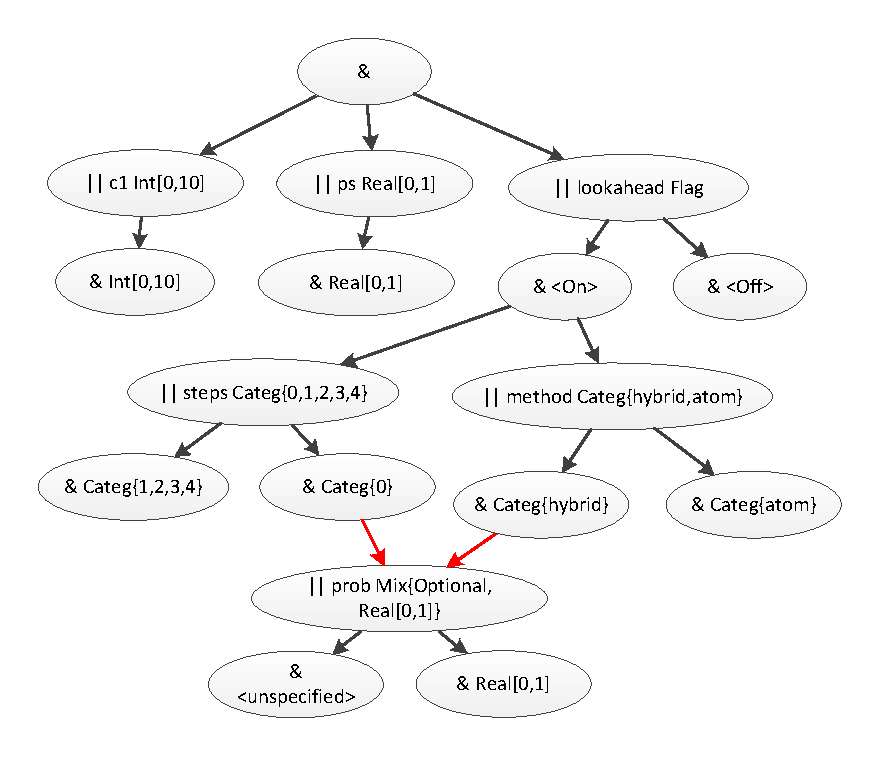
\includegraphics[width=10cm]{paramgraph.pdf}
\end{figure}

The two red edges imply the membership of the edges to the same edge group $\neq 0$. Black edges mean that the edge doesn't belong to any group.
For simplicity, the parameter references of AND-Nodes (to the same parameter as the preceeding OR-Node) are not shown in the graph.
\clearpage
\subsection{Implementation etc.}
\begin{itemize}
\item define parameter graphs in XML / GUI 
\item API documentation for configurators
\end{itemize}